\documentclass[serif, 12pt]{beamer}

\usepackage{graphicx} % Allows including images
\usepackage{booktabs} % Allows the use of \toprule, \midrule and \bottomrule in tables

\usepackage{algorithm2e}
\usepackage{hyperref}

\newcommand*\mat[1]{ \begin{pmatrix} #1 \end{pmatrix}}
\newcommand*\arr[1]{ \begin{bmatrix} #1 \end{bmatrix}}
\newcommand*\V[1]{ \boldsymbol{#1}}

\setbeamertemplate{navigation symbols}{}%remove navigation symbols

\title{Approximated PCA}

\author{Rodrigo Arias} % Your name
\date{\today} % Date, can be changed to a custom date

\begin{document}

\begin{frame}
	\titlepage
\end{frame}

%------------------------------------------------

\begin{frame}

\frametitle{PCA algorithm}

\begin{enumerate}
\item Take a dataset $X$.
\item Scale and center the variables.
\item From $X$ compute the covariance matrix $S$.
\item \textbf{Compute the eigenvalues and eigenvectors of $S$.}
\item \textit{Optional: Ignore some eigenvectors.}
\item Generate a new basis from the selected eigenvectors.
\item Project $X$ into the new basis.
\end{enumerate}

\pause

Computing the eigenvectors is the principal step of PCA.

\end{frame}

%------------------------------------------------

\begin{frame}

\frametitle{Visual example}
The input dataset with 800 variables $X$ = 

\begin{center}
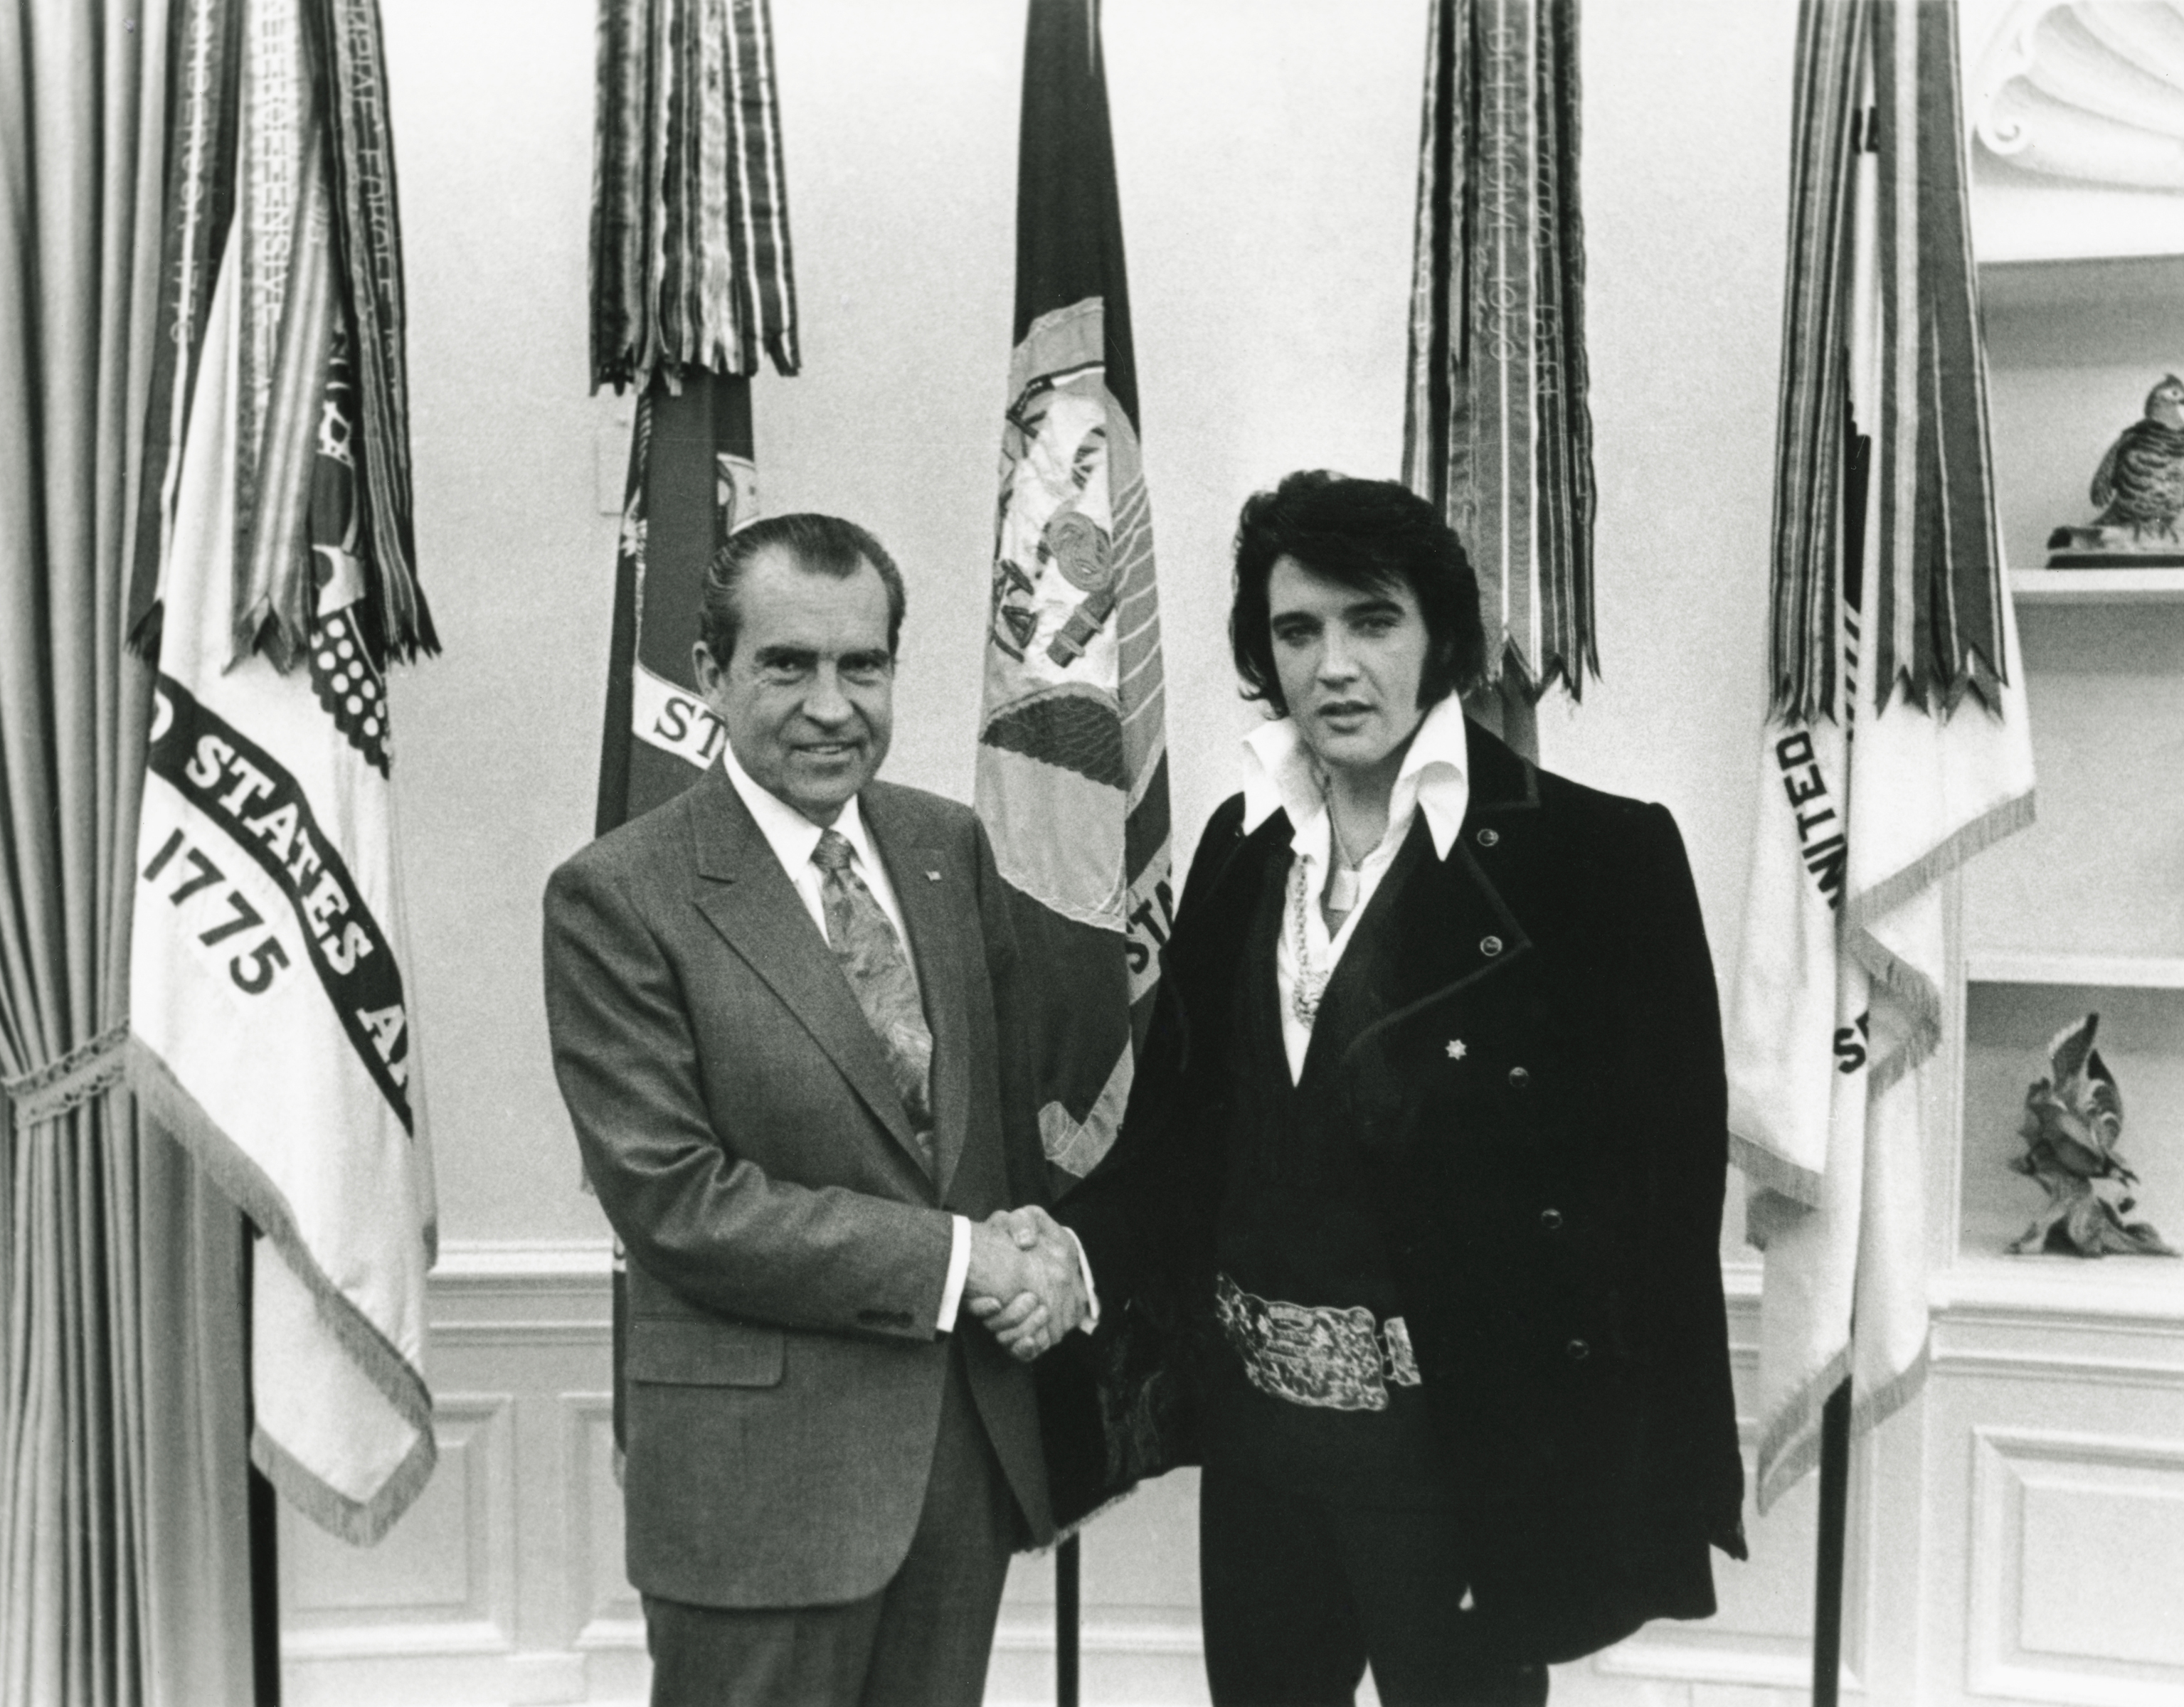
\includegraphics[width=\textheight]{input}
\end{center}

\end{frame}

%------------------------------------------------

\begin{frame}

\frametitle{Visual example}
Keep 200 eigenvectors. Output:

\begin{center}
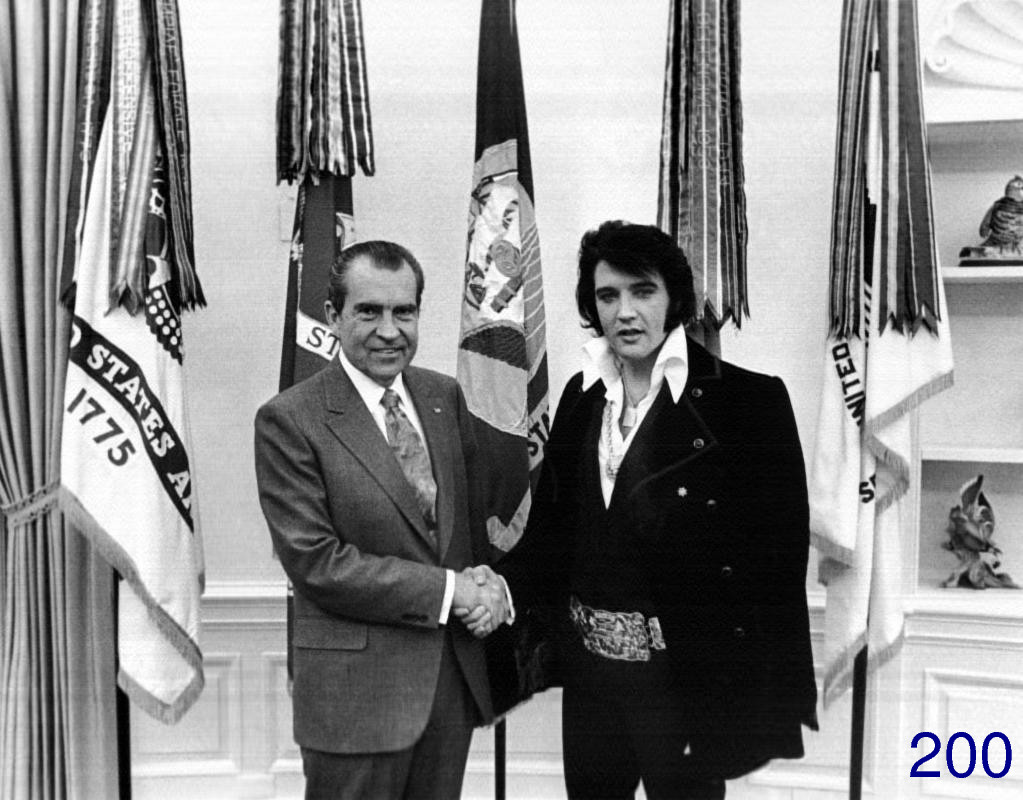
\includegraphics[width=\textheight]{out-200}
\end{center}

\end{frame}

%------------------------------------------------

\begin{frame}

\frametitle{Visual example}
Keep 100 eigenvectors. Output:

\begin{center}
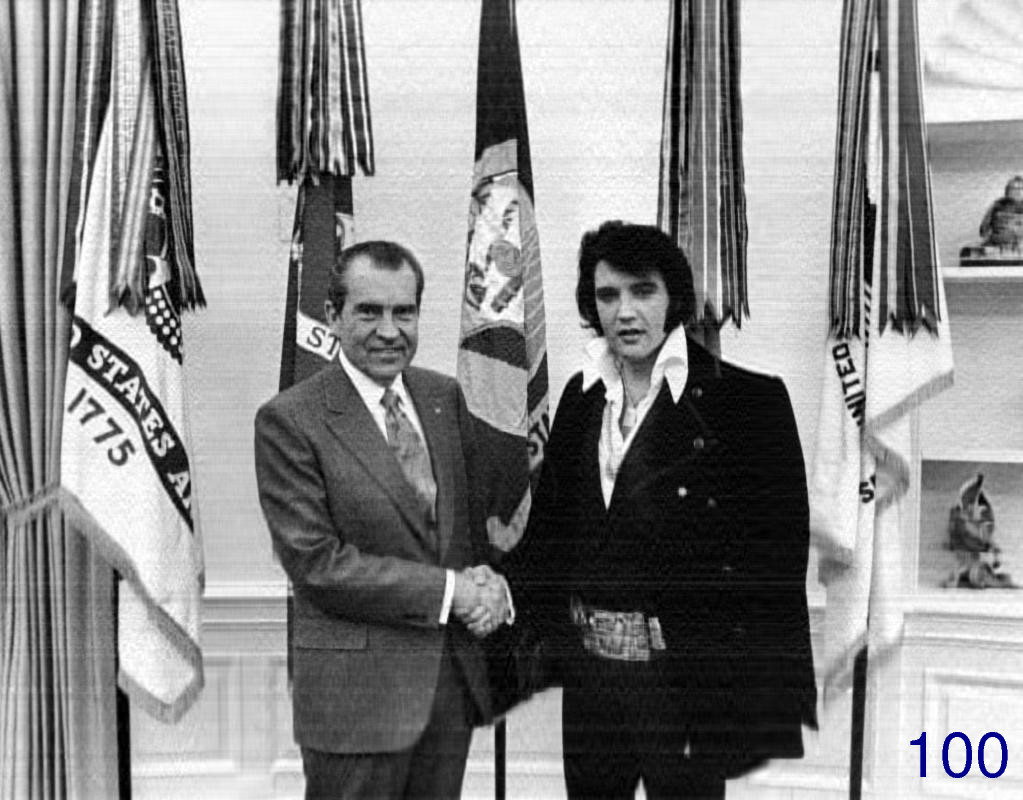
\includegraphics[width=\textheight]{out-100}
\end{center}

\end{frame}

%------------------------------------------------

\begin{frame}

\frametitle{Visual example}
Keep 40 eigenvectors. Output:

\begin{center}
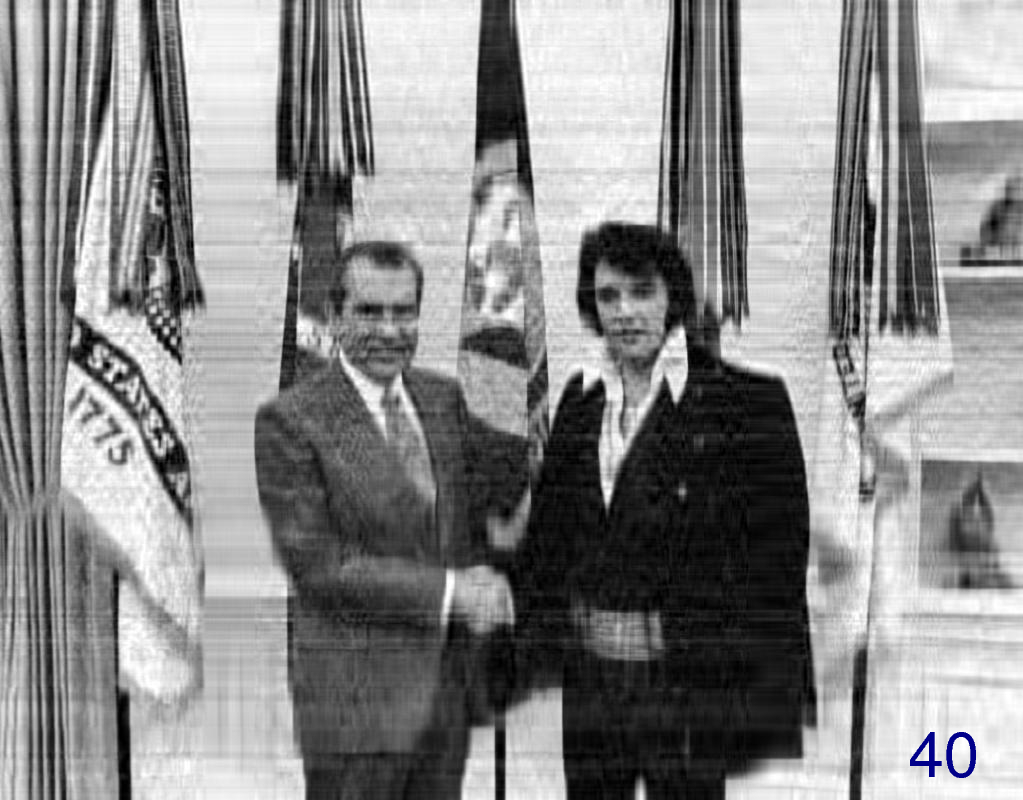
\includegraphics[width=\textheight]{out-40}
\end{center}

\end{frame}

%------------------------------------------------

\begin{frame}

\frametitle{Computing eigenvalues and eigenvectors}

\begin{enumerate}
\item Take the target matrix $A$.
\item Compute a tridiagonal matrix $T$, $A = PTP^T$.
\item From $T$ compute a diagonal matrix $D$, $T = QTQ^T$.
\item The eigenvalues of $A$ are in the diagonal of $D$.
\item Compute the eigenvectors from $D$.
\end{enumerate}

\pause

Computing a tridiagonal matrix is called \textbf{tridiagonalization}. For the 
diagonal, \textbf{diagonalization}. Several algorithms exists for both steps.

\end{frame}


%------------------------------------------------

\begin{frame}
%
\frametitle{Tridiagonalization}
%
These algorithms transform a \textbf{symmetric} matrix $A$ into a new pair of 
matrices $P$ and $T$ such that $P$ is orthogonal, $T$ is tridiagonal, and $A = 
PTP^T$
%
$$
	\mat{
		a_{11} & a_{12} & a_{13} & a_{14} \\
		a_{21} & a_{22} & a_{23} & a_{24} \\
		a_{31} & a_{32} & a_{33} & a_{34} \\
		a_{41} & a_{42} & a_{43} & a_{44} \\
	} =
	Q
	\mat{
		t_{11} & t_{12} &        &        \\
		t_{21} & t_{22} & t_{23} &        \\
		       & t_{32} & t_{33} & t_{34} \\
		       &        & t_{43} & t_{44} \\
	}
	Q^T
$$
%
\end{frame}

%------------------------------------------------

\begin{frame}
%
\frametitle{Tridiagonalization}
%
\begin{center}
\begin{tabular}{c c c c}
	\toprule
	Algorithm 		& Complexity  & Iterative & Stability\\
	\midrule
	Householder		& $O(4n^3/3)$ & No        & Great\\
	Givens				& $O(kn^3)$   & No        & Good \\
	Lanczos				& $O(kpn^2)$  & Yes       & Bad \\
	Others				&             &          \\
	\bottomrule
\end{tabular}
\end{center}
Where $k$ is some constant, and $p$ the number of iterations.
\end{frame}

%------------------------------------------------

\begin{frame}
%
\frametitle{Diagonalization}
%
These algorithms take a \textbf{tridiagonal} matrix $T$ into a new pair of 
matrices $Q$ and $D$ such that $Q$ is orthogonal, $D$ is diagonal, and $T = 
QDQ^T$
%
$$
	\mat{
		t_{11} & t_{12} &        &        \\
		t_{21} & t_{22} & t_{23} &        \\
		       & t_{32} & t_{33} & t_{34} \\
		       &        & t_{43} & t_{44} \\
	}=
	Q
	\mat{
		d_{11} &        &        &        \\
		       & d_{22} &        &        \\
		       &        & d_{33} &        \\
		       &        &        & d_{44} \\
	}
	Q^T
$$
%
The matrix $D$ contains the \textbf{eigenvalues} in the diagonal.
\end{frame}

%------------------------------------------------

\begin{frame}
%
\frametitle{Diagonalization}
%
\begin{center}
\begin{tabular}{c c c c}
	\toprule
	Algorithm 		& Complexity  & Iterative & Convergence\\
	\midrule
	QR                  & $O(6n^3)$ 	& Yes       & Cubic \\
	Divide and conquer  & $O(8n^3/3)$ & Yes       & Quadratic \\
	Jacobi              & $O(n^3)$    & Yes       & Quadratic \\
	Power iteration			& $O(n^3)$    & Yes       & Linear \\
	Inverse iteration	  & $O(n^3)$    & Yes       & Linear \\
	Others				&             &          \\
	\bottomrule
\end{tabular}
\end{center}
\end{frame}

%------------------------------------------------

\begin{frame}
%
\frametitle{The selected method}
%
\centering
Householder + QR
\end{frame}

%------------------------------------------------


\end{document}
